\section{Principles of Quantum Physics}
In this section, we will introduce the principles in an axiomatic form. We will formulate them in algebraic manner appropriate for quantum information and computation in finite dimensional Hilbert space.
\begin{parag}{Hilbert space}
Note here that we have not defined what a Hilbert space here is so let me define it (wikipedia)
\begin{definition}{(Hilbert Space)}
A \important{Hilbert} space is a real or complex inner product space that is also a complete metric space with respect to the distance function induced by the inner product
\end{definition}
To say that a complex vector space $\mathcal{H}$ is a complex inner product space means that there is an inner product $\langle x, y\rangle$ associating a complex number to each pair of elements $x, y$ of $\mathcal{H}$ that satisfies the following properties:
\begin{enumerate}
    \item The inner product is conjugate symmetric; that is the inner product of a pair of elements is equal to the complex conjugate of the inner product of the swapped elements:
	\begin{align*} 
		\langle y, x\rangle = \overline{\langle x, y\rangle} 
	\end{align*}
	Importantly, this implies that $\langlex, x\rangle$ is a real number
	\item The inner product is linear in its first argument. For all complex number $a, b \in\mathbb{C}$
		\begin{align*} 
			\langle ax_1 + bx_2, y\rangle  = a\langle x_1, y\rangle + b\langle x_2, y\rangle
		\end{align*}
	\item The inner product of an element with itself is positive definite 
		\begin{align*} 
			\langle x, x\rangle &> 0 \mathspace \mathspace \text{ if } x \neq 0\\
			 \langle x, x\rangle &=  0 \mathspace \mathspace \text{ if } x = 0
		\end{align*}
\end{enumerate}


\end{parag}

\subsection{Principle 1: State vectors}

The state of a physical system can be described (isolated from the rest of the universe) as a vector in a finite dimensional Hilbert space $\mathcal{H}$, we denote it as
\begin{align*} 
	\ket{\psi} \in \mathcal{H} 
\end{align*}
This vector $\ket{\psi}$ must be normalized with respect to the inner product of that Hilbert space, meaning $\braket{\psi}{\psi} = 1$.
\begin{framedremark}
The principle doesn't say how to choose $\ket{\psi}$ neither the space itself $\mathcal{H}$. This decision comes from the underlying physics of the system.
\end{framedremark}
\begin{framedremark}
In a non-isolated system we will have to generalize this principle. This will be done in later part of the course when introducing the notion of \important{density} matrix.
\end{framedremark}
    Hence let us start with the most basic example in quantum physics, the qbit! The Hilbert space describing a qbit is given as $\mathcal{H} = \mathbb{C}^2$ which can be denoted as 
	\begin{align*} 
		\mathcal{H} = \mathbb{C}^2 &= \left\{\begin{pmatrix} \alpha \\ \beta \end{pmatrix}, \alpha, \beta \in \mathbb{C} \right\} \\
								   &= \left\{\alpha \ket{0} + \beta\ket{1}, \alpha \in \mathbb{C}, \beta \in \mathbb{C}\right\}
	\end{align*}
	Furthermore for this state to be correctly the state of a qbit it also must satisfy normalization, meaning its norm is 1. Recall not the definition of the inner product of a Hilbert space did we even define our inner product here? Recall that we need to validate the three properties above, a valid choice here is the following inner product:
	\begin{align*} 
		\langle x, y\rangle  = \sum_{i= 1}^{n} x_i^{\ast}y_i
	\end{align*}
	You can check that this inner product here fulfils all properties. Going back on our requirement ($\left\|x\right\| = 1$) we will therefore need
	\begin{align*} 
		\alpha^\ast\alpha + \beta^\ast\beta = 1
	\end{align*}
	With that requirement, we have the Hilbert space of a qbit.\\
	$ $\\
	Also in terms of notation, we will often use the letter $\psi$, $\varphi$ and $ \phi$ in order to represent quantum states. We will also use the term state to refer to quantum state as all work here is primarily done in the quantum world. Hence we define our qbit as 
	\begin{align*} 
		\ket{\psi} = \alpha \ket{0} + \beta \ket{1} 
	\end{align*}
	For more general states, ones of dimension $d$ (i.e. $\mathcal{H} = \mathbb{C}^{d}$) our state is constructed as 
	\begin{align*} 
		\ket{\psi} = \sum_{i= 1}^{d} \alpha_i \ket{i}
	\end{align*}
	\begin{framedremark}
	    Note that state doesn't have to be necessarily finite. A good example of this are quantum harmonic oscillators (so PHYS-344) in which our state is defined as 
		\begin{align*} 
			 \ket{\Psi} = \sum_{n= 0}^{\infty} \psi_n \ket{n}
		\end{align*}
	\end{framedremark}



\subsection{Principle 2: Unitary evolution on time evolution}
The state of an isolated system evolves (as a function of time) unitarily. This means that of $\ket{\psi_0}$ is a state at time $= 0$, the state $\ket{\psi_t}$ is given by 
\begin{align*} 
	U_t \ket{\psi_0}  = \ket{\psi_t}
\end{align*}
Where $U_t^{\dagger}U_t = U_tU_t^{\dagger} = I$ i.e. $U_t$ is unitary (usually time dependent) matrix
\begin{framedremark}
One can show that unitary matrix represent rotation of the space by a specified angles.
\end{framedremark}

\begin{framedremark}
	For people of have done or who are doing MATH-310 (Algebra), one can see that the time evolution matrices form a group in the sense that 
	\begin{align*} 
		U_{t_2}U_{t_1} U_{t_1 + t_2} \mathspace \mathspace , U_{t= 0} = I
	\end{align*}
\end{framedremark}


\begin{parag}{Example}
    Let us take the example of a reflecting mirror :
	\begin{center}
	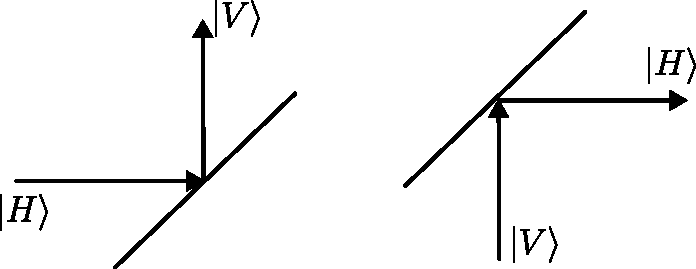
\includegraphics[width=0.6\textwidth]{figure/2026-10-19.pdf}
	\end{center}
	The physical process which transforms the incident ray into the reflected ray is described by the unitary matrix:
	\begin{align*} 
		X = \begin{pmatrix} 0 & 1 \\ 1 & 0 \end{pmatrix}  = \ket{H}\bra{V} + \ket{V}\bra{H}
	\end{align*}
	For $\ket{H}= \begin{pmatrix} 1 \\ 0 \end{pmatrix} $ and $\ket{V} = \begin{pmatrix} 0 \\ 1 \end{pmatrix} $. Let us take a step back on what is actually going on here. What a perfectly reflecting mirror with a tilted angle here reflect a ray that is normal  ($\braket{\psi_{t_1}}{\psi_{t_2}} = 0$) for the state after and before the mirror, so here we would require that $U\ket{H} = \ket{V}$ and vis versa which if you apply $X$ on any of those two states gives the intended results.
\end{parag}




